% Options for packages loaded elsewhere
\PassOptionsToPackage{unicode}{hyperref}
\PassOptionsToPackage{hyphens}{url}
%
\documentclass[
  12pt,
]{article}
\usepackage{amsmath,amssymb}
\usepackage{lmodern}
\usepackage{iftex}
\ifPDFTeX
  \usepackage[T1]{fontenc}
  \usepackage[utf8]{inputenc}
  \usepackage{textcomp} % provide euro and other symbols
\else % if luatex or xetex
  \usepackage{unicode-math}
  \defaultfontfeatures{Scale=MatchLowercase}
  \defaultfontfeatures[\rmfamily]{Ligatures=TeX,Scale=1}
\fi
% Use upquote if available, for straight quotes in verbatim environments
\IfFileExists{upquote.sty}{\usepackage{upquote}}{}
\IfFileExists{microtype.sty}{% use microtype if available
  \usepackage[]{microtype}
  \UseMicrotypeSet[protrusion]{basicmath} % disable protrusion for tt fonts
}{}
\makeatletter
\@ifundefined{KOMAClassName}{% if non-KOMA class
  \IfFileExists{parskip.sty}{%
    \usepackage{parskip}
  }{% else
    \setlength{\parindent}{0pt}
    \setlength{\parskip}{6pt plus 2pt minus 1pt}}
}{% if KOMA class
  \KOMAoptions{parskip=half}}
\makeatother
\usepackage{xcolor}
\IfFileExists{xurl.sty}{\usepackage{xurl}}{} % add URL line breaks if available
\IfFileExists{bookmark.sty}{\usepackage{bookmark}}{\usepackage{hyperref}}
\hypersetup{
  pdftitle={Appendix S1: Supporting Tables and Figures.},
  hidelinks,
  pdfcreator={LaTeX via pandoc}}
\urlstyle{same} % disable monospaced font for URLs
\usepackage[margin=1in]{geometry}
\usepackage{longtable,booktabs,array}
\usepackage{calc} % for calculating minipage widths
% Correct order of tables after \paragraph or \subparagraph
\usepackage{etoolbox}
\makeatletter
\patchcmd\longtable{\par}{\if@noskipsec\mbox{}\fi\par}{}{}
\makeatother
% Allow footnotes in longtable head/foot
\IfFileExists{footnotehyper.sty}{\usepackage{footnotehyper}}{\usepackage{footnote}}
\makesavenoteenv{longtable}
\usepackage{graphicx}
\makeatletter
\def\maxwidth{\ifdim\Gin@nat@width>\linewidth\linewidth\else\Gin@nat@width\fi}
\def\maxheight{\ifdim\Gin@nat@height>\textheight\textheight\else\Gin@nat@height\fi}
\makeatother
% Scale images if necessary, so that they will not overflow the page
% margins by default, and it is still possible to overwrite the defaults
% using explicit options in \includegraphics[width, height, ...]{}
\setkeys{Gin}{width=\maxwidth,height=\maxheight,keepaspectratio}
% Set default figure placement to htbp
\makeatletter
\def\fps@figure{htbp}
\makeatother
\setlength{\emergencystretch}{3em} % prevent overfull lines
\providecommand{\tightlist}{%
  \setlength{\itemsep}{0pt}\setlength{\parskip}{0pt}}
\setcounter{secnumdepth}{-\maxdimen} % remove section numbering
\newlength{\cslhangindent}
\setlength{\cslhangindent}{1.5em}
\newlength{\csllabelwidth}
\setlength{\csllabelwidth}{3em}
\newlength{\cslentryspacingunit} % times entry-spacing
\setlength{\cslentryspacingunit}{\parskip}
\newenvironment{CSLReferences}[2] % #1 hanging-ident, #2 entry spacing
 {% don't indent paragraphs
  \setlength{\parindent}{0pt}
  % turn on hanging indent if param 1 is 1
  \ifodd #1
  \let\oldpar\par
  \def\par{\hangindent=\cslhangindent\oldpar}
  \fi
  % set entry spacing
  \setlength{\parskip}{#2\cslentryspacingunit}
 }%
 {}
\usepackage{calc}
\newcommand{\CSLBlock}[1]{#1\hfill\break}
\newcommand{\CSLLeftMargin}[1]{\parbox[t]{\csllabelwidth}{#1}}
\newcommand{\CSLRightInline}[1]{\parbox[t]{\linewidth - \csllabelwidth}{#1}\break}
\newcommand{\CSLIndent}[1]{\hspace{\cslhangindent}#1}
\usepackage{float}
\usepackage{booktabs}
\usepackage{colortbl}
\usepackage{fancyhdr}
\pagestyle{fancy}
\usepackage[default]{sourcesanspro}
\usepackage{sourcecodepro}
\fancypagestyle{plain}{\pagestyle{fancy}}
\fancyhead[RE,RO]{Maenpuen \textit{et al}. --American Journal of Botany-- Appendix S1}
\usepackage{booktabs}
\usepackage{longtable}
\usepackage{array}
\usepackage{multirow}
\usepackage{wrapfig}
\usepackage{float}
\usepackage{colortbl}
\usepackage{pdflscape}
\usepackage{tabu}
\usepackage{threeparttable}
\usepackage{threeparttablex}
\usepackage[normalem]{ulem}
\usepackage{makecell}
\usepackage{xcolor}
\ifLuaTeX
  \usepackage{selnolig}  % disable illegal ligatures
\fi

\title{Appendix S1: Supporting Tables and Figures.}
\author{}
\date{\vspace{-2.5em}}

\begin{document}
\maketitle

{
\setcounter{tocdepth}{2}
\tableofcontents
}
\newpage

\hypertarget{table-s1}{%
\section{Table S1:}\label{table-s1}}

Site information.
MAT: mean annual temperature,
MAP: mean annual precipitation,
CV: coefficient of variation.

\begin{table}[H]
\centering
\begin{tabular}[t]{>{\raggedright\arraybackslash}p{3cm}>{\raggedright\arraybackslash}p{3cm}>{\raggedright\arraybackslash}p{3cm}>{\raggedright\arraybackslash}p{3cm}>{\raggedright\arraybackslash}p{3cm}}
\toprule
  & Bubeng & Ailao-shan & Yuanjiang & Yakushima\\
\midrule
\cellcolor{gray!6}{Site name} & \cellcolor{gray!6}{Yunnan} & \cellcolor{gray!6}{Yunnan} & \cellcolor{gray!6}{Yunnan} & \cellcolor{gray!6}{Yakushima}\\
Vegetation & Tropical forest (TRF) & Subtropical evergreen wet forest (STF) & Hot-dry savanna  (HDS) & Warm-temperate forest\\
\cellcolor{gray!6}{Elevation (m)} & \cellcolor{gray!6}{780} & \cellcolor{gray!6}{2500} & \cellcolor{gray!6}{480} & \cellcolor{gray!6}{14 - 1748}\\
Location & 21°37'N, 101°35'E & 24°32'N, 101°01'E & 23°28'N, 102°10'E & 30°38'N, 130°62'E\\
\cellcolor{gray!6}{MAT (℃)} & \cellcolor{gray!6}{21} & \cellcolor{gray!6}{11.7} & \cellcolor{gray!6}{24.7} & \cellcolor{gray!6}{8.1 - 19.4}\\
\addlinespace
MAP (mm) & 1532.0 & 1931.0 & 732.8 & 4477.0\\
\cellcolor{gray!6}{Dry period (month)} & \cellcolor{gray!6}{6} & \cellcolor{gray!6}{-} & \cellcolor{gray!6}{6} & \cellcolor{gray!6}{-}\\
Canopy height (m) & 35-45 & 25 & 4-6 & -\\
\cellcolor{gray!6}{Leaf thickness} & \cellcolor{gray!6}{Measured} & \cellcolor{gray!6}{Measured} & \cellcolor{gray!6}{Measured} & \cellcolor{gray!6}{Measured}\\
Leaf disc thickness & Measured & Measured & Measured & Not-measured\\
\addlinespace
\cellcolor{gray!6}{Leaf punch diameter (cm)} & \cellcolor{gray!6}{0.6} & \cellcolor{gray!6}{0.6} & \cellcolor{gray!6}{0.6} & \cellcolor{gray!6}{1.0}\\
Number of species for species means & 60 & 47 & 34 & 193\\
\cellcolor{gray!6}{Number of individuals for individuals means} & \cellcolor{gray!6}{366} & \cellcolor{gray!6}{282} & \cellcolor{gray!6}{204} & \cellcolor{gray!6}{607}\\
Number of species for CV & 60 & 47 & 33 & 5\\
\cellcolor{gray!6}{Number of individuals for CV} & \cellcolor{gray!6}{366} & \cellcolor{gray!6}{282} & \cellcolor{gray!6}{203} & \cellcolor{gray!6}{26}\\
\bottomrule
\end{tabular}
\end{table}

The site information and climate data in Yunnan, referred to Fei et al. (\protect\hyperlink{ref-Fei2018}{2018}), and Song et al. (\protect\hyperlink{ref-Song2017}{2017}).
MAT and MAP of Yakushima were obtained from the Yakushima meteorological station and Eguchi (\protect\hyperlink{ref-Eguchi2006}{2006}).

\newpage

\hypertarget{table-s2}{%
\section{Table S2:}\label{table-s2}}

Summary of a linear mixed model for log-transformed total dry mass of leaf discs for each tree individual.
Species was used as a random intercept.
The leaf punch size is described as an effect of `0.6 cm diameter' compared with `1.0 cm diameter'.

\begin{table}[H]
\centering
\begin{tabular}[t]{rrrrl}
\toprule
Estimate & SE & DF & t-value & \textit{P} value\\
\midrule
\cellcolor{gray!6}{-4.410} & \cellcolor{gray!6}{0.013} & \cellcolor{gray!6}{1030} & \cellcolor{gray!6}{-333.00} & \cellcolor{gray!6}{< 0.001}\\
0.240 & 0.007 & 1030 & 33.20 & < 0.001\\
\cellcolor{gray!6}{-0.061} & \cellcolor{gray!6}{0.009} & \cellcolor{gray!6}{1030} & \cellcolor{gray!6}{-6.94} & \cellcolor{gray!6}{< 0.001}\\
0.277 & 0.008 & 1030 & 34.90 & < 0.001\\
\cellcolor{gray!6}{-0.500} & \cellcolor{gray!6}{0.020} & \cellcolor{gray!6}{332} & \cellcolor{gray!6}{-25.60} & \cellcolor{gray!6}{< 0.001}\\
\bottomrule
\end{tabular}
\end{table}

\newpage

\hypertarget{figure-s1}{%
\section{Figure S1:}\label{figure-s1}}

Detailed sampling protocol for whole-leaf and leaf disc LMA.

\begin{center}
\includegraphics[width=4.89583in,height=\textheight]{../figs/S2.jpeg}

\end{center}

\newpage

\hypertarget{figure-s2}{%
\section{Figure S2:}\label{figure-s2}}

Generalization for a relationship between ratios of disc-based and whole-leaf estimates of leaf mass per area (LMA), leaf tissue density (LD), and leaf thickness (LT).
For the \emph{i} tree individual or species, the relationship between ratios of disc-based and whole-leaf estimates of LMA, LD, and LT is:

\[
\frac{LDd_i}{LDw_i} = \frac{LMAd_i}{LMAw_i} \frac{LTw_i}{LTd_i}
\]

where \emph{d} indicates disc-based estimates, \emph{w} indicates whole-leaf based estimates.

Because thickness is measured on leaf lamina whether one uses a leaf disc or a whole-leaf, the expected ratio between thickness for a leaf disc and a whole-leaf should be 1.
The above relationship, therefore, can be rewritten using lognormally distributed multiplicative error (\(\epsilon_i\)) on the arithmetic scale:

\[
\frac{LDd_i}{LDw_i} = \frac{LMAd_i}{LMAw_i} exp(\epsilon_i) \;\;\;\;\epsilon_i \sim N(0, \sigma^2).
\]

LMA requires two times measurements (mass and area) and LD requires three time measurements (mass, area and thickness), and thus variance in the ratio of whole-leaf LD and leaf disc LD should be greater than that of LMA.

As we expected LD, showed the slightly smaller \emph{R\textsuperscript{2}} value than LMA (Figure below) in the Yunnan dataset.
We have independent measurement for thickness for leaf discs and whole-leaves in the Yunnan dataset.
If we use the same leaf thickness values for leaf discs and whole-leaves (i.e., LTw\textsubscript{i}/LTd\textsubscript{i} =1), the scatter plots will be identical for LMA and LD.
Consequently, we do not perform further analyses for LD, because differences between whole-leaf LD and leaf disc LD only depends on the ratio between whole-leaf LMA and leaf disc LMA and measurement errors of leaf thickness.

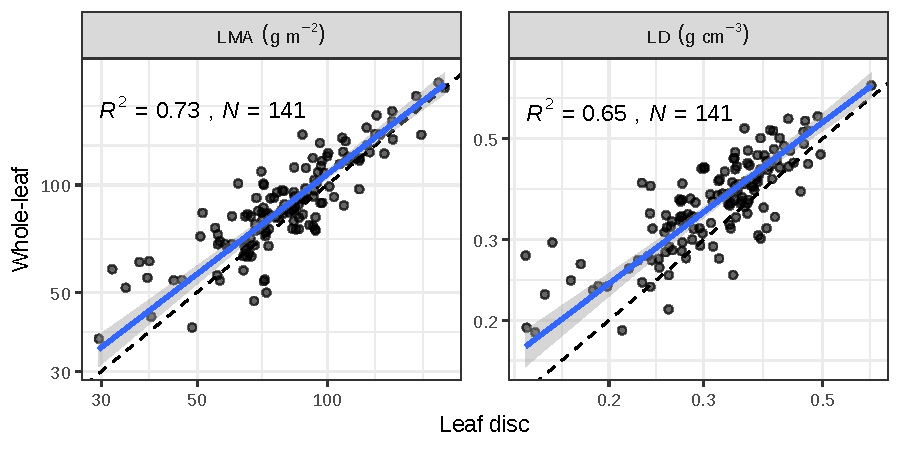
\includegraphics[width=6.25in,height=\textheight]{../figs/lma_ld.pdf}

Relationships between species mean leaf mass per area (LMA) and leaf tissue density (LD) determined by using whole leaves and leaf discs for the Yunnan dataset that has both leaf thickness for leaf discs and whole leaves.
Dashed lines indicate 1:1 lines.
Blue solid lines indicate standardized major axis regressions.
The 95\% confidence intervals are presented as the shaded area.
All the correlations are significant (\emph{P} \textless{} 0.001).

\newpage

\hypertarget{figure-s3}{%
\section{Figure S3:}\label{figure-s3}}

Standardized regression coefficients modelig the effects of leaf tissue density,
leaf area,
leaf thickness,
punch size, and
their interactios
(a) on the mean estimates of whole-leaf LMA, and
(b) on the estimated variance of whole-leaf LMA.
The leaf disc LMA was used for the baseline mean of the whole-leaf LMA.
Thick and thin lines indicate 90\% and 95\% credible intervals, respectively.
Circles show posterior means of coefficients.
Circles filled with blue indicate significant effects and white indicate non-significance effects.

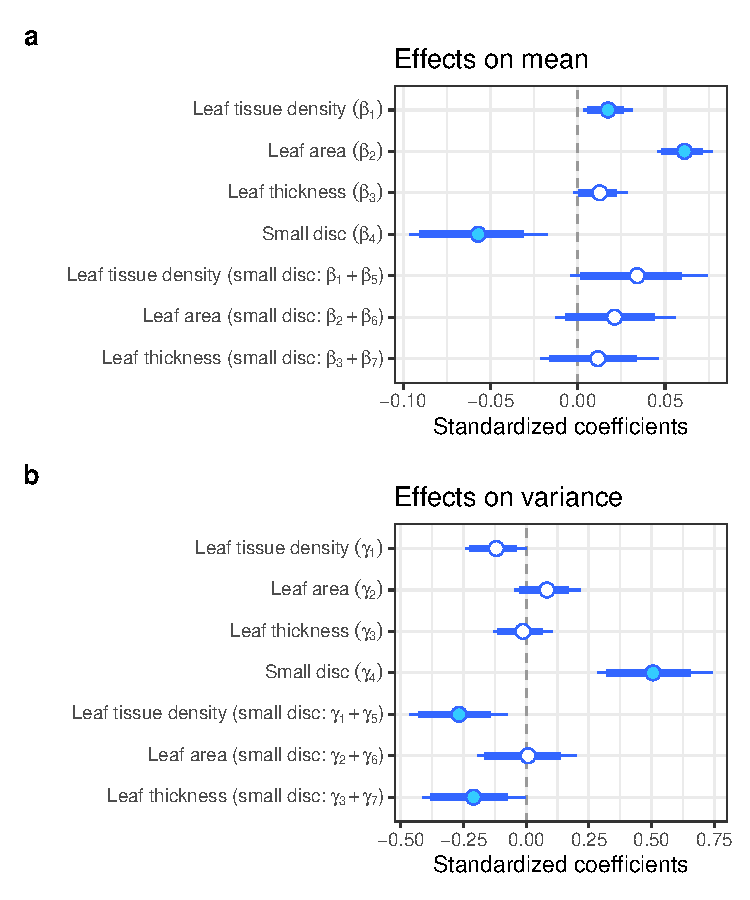
\includegraphics{../figs/coef_sp_punch1_add.pdf}

\newpage

\hypertarget{figure-s4}{%
\section{Figure S4:}\label{figure-s4}}

Relationships between species mean leaf mass per area (LMA) determined by using whole-leaves and leaf discs for species obtained with leaf punches of different diameters.
Dashed lines indicate 1:1 lines.
Blue solid lines indicate standardized major axis (SMA) regressions.
The 95\% confidence intervals are resented as the shaded area.
The correlation is significant (\emph{P} \textless{} 0.001).

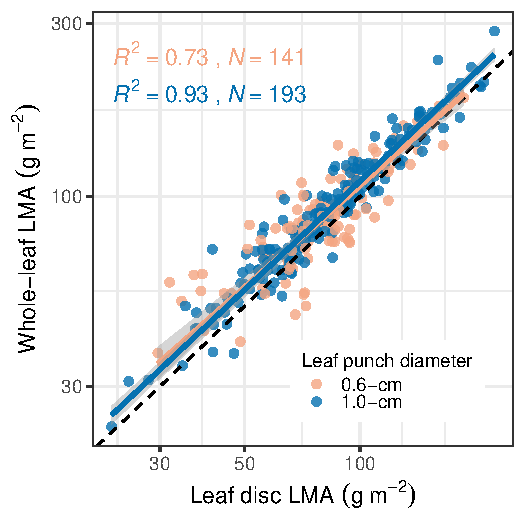
\includegraphics[width=4.16667in,height=\textheight]{../figs/sma_sep.pdf}

\newpage

\hypertarget{figure-s5}{%
\section{Figure S5:}\label{figure-s5}}

Relationships between whole-leaf LMA : disc leaf LMA and total dry mass for the leaf disc.
The relationships was heteroscedastic (unequal variance, \emph{p} \textless{} 0.001; all the samples were analyzed together).
Samples with small total dry mass tended to show greater variance.

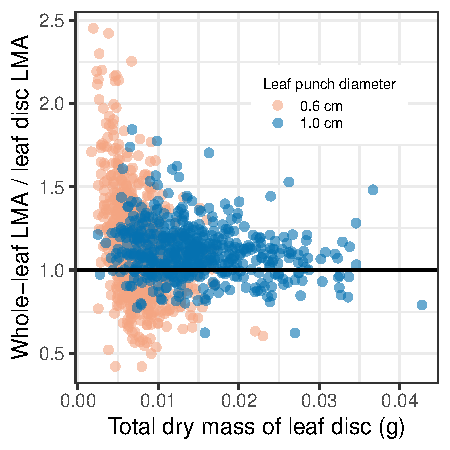
\includegraphics[width=4.16667in,height=\textheight]{../figs/ratio_dm.pdf}

\newpage

\hypertarget{literature-cited}{%
\section*{LITERATURE CITED}\label{literature-cited}}
\addcontentsline{toc}{section}{LITERATURE CITED}

\hypertarget{refs}{}
\begin{CSLReferences}{1}{0}
\leavevmode\vadjust pre{\hypertarget{ref-Eguchi2006}{}}%
Eguchi, T. 2006. Climate. Yakushima, 3--26. {Asakura Shoten}, {Tokyo (in Japanese)}.

\leavevmode\vadjust pre{\hypertarget{ref-Fei2018}{}}%
Fei, X., Q. Song, Y. Zhang, Y. Liu, L. Sha, G. Yu, L. Zhang, et al. 2018. \href{https://doi.org/10.1016/j.scitotenv.2017.10.239}{Carbon exchanges and their responses to temperature and precipitation in forest ecosystems in {Yunnan}, {Southwest China}}. \emph{Science of The Total Environment} 616--617: 824--840.

\leavevmode\vadjust pre{\hypertarget{ref-Song2017}{}}%
Song, Q. H., Y. P. Zhang, L. Q. Sha, X. B. Deng, Y. Deng, C. S. Wu, Z. Y. Lu, et al. 2017. \href{https://doi.org/10.3832/ifor2223-010}{Canopy temperature variability in a tropical rainforest, subtropical evergreen forest, and savanna forest in {Southwest China}}. \emph{iForest - Biogeosciences and Forestry} 10: 611.

\end{CSLReferences}

\end{document}
